\chapter{Facility Airside Operation and Design Overview}
\label{ch:Facility Airside Operation and Design Overview}

\section{Explanation of Facility Operation}
\label{sec:Explanation of Facility Operation}

Before listing the criteria and limits used to design the facility, it is beneficial to describe how the airside cycle within the facility will operate. The closed-loop airside subsystem contains the tested heat exchanger coil, along with an airflow measurement apparatus (i.e. code tester) and the necessary conditioning equipment to recirculate air and achieve the desired set point condition at the inlet of the tested coil. As air flows over the tested coil in the test section, the thermodynamic properties of air are modified through heat addition or rejection. Using the conditioning section, the air properties are then returned to the desired set point conditions before returning to the inlet of the tested coil. A schematic of the airside subsystem can be seen in Figure \ref{fig:TunnelAirsideSchematic}.

\begin{figure}[h!]
    \centering
    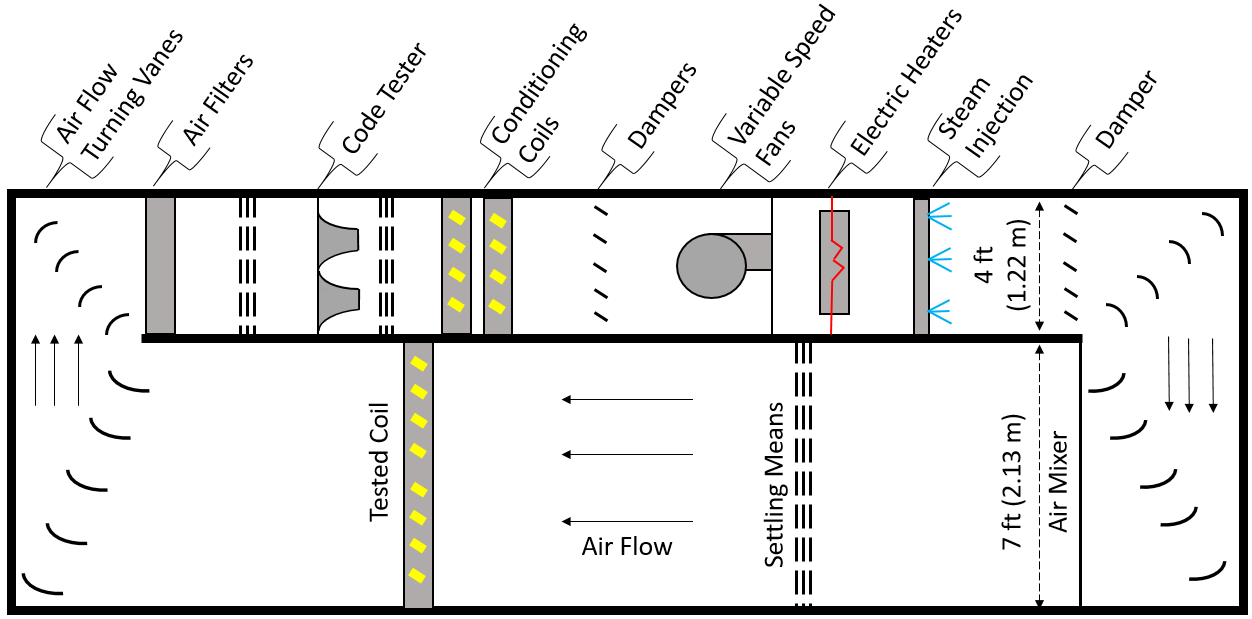
\includegraphics[width=1\textwidth]{TunnelAirsideSchematic}
    \caption{Simplified schematic of airside schematic with major components identified}
    \label{fig:TunnelAirsideSchematic}
\end{figure}

Air travels through the tested coil, where properties are changed through heat addition, heat rejection, and/or dehumidification depending on the experiment. From the exit of the tested coil, the air flows through two sets of turning vanes and enters the conditioning section of the facility. The conditioning section contains a series combination of air filters, a code tester, conditioning coils, variable speed fans, electric reheat, steam humidification, and dampers. The air filters prevent any large debris or contaminants from entering subsequent conditioning equipment. The code tester allows for the calculation of airflow rate. It contains a nozzle plane with upstream and downstream air settling means, placed according to ASHRAE Standard 41.2 (2018) specifications. Four conditioning coils, arranged vertically into two pairs, counteract the change in air properties that occurred at the test coil by conditioning the air. A pair of dampers, downstream of the conditioning coils, determine which conditioning coil(s) air crosses over. Each coil can independently operate in heating or cooling mode. Variable speed fans provide the pressure rise needed to pass the air throughout the airside loop. Electric heaters provide reheat and are intended for precise air temperature control. Humidity control is achieved by a steam humidifier and injection manifold, allowing moisture to be reintroduced to the airstream. The damper located after the steam injection allows operation at reduced airflow rates by increasing static pressure on the fans. Upon leaving the conditioning section, air is returned to the test section via turning vanes. Air is then mixed to reduce temperature and humidity stratification throughout the cross section of the test section. Finally, a set of settling means creates a more uniform air velocity distribution before again arriving at the inlet of the tested coil.

\section{Design Operating Envelope}
\label{sec: Design Operating Envelope}

With a basic understanding of how the facility airside will operate, it is necessary to determine the physical size of the facility, as well as the limits of operation for set point conditions. Commercial size heat exchanger coils are the primary type of coil to be tested in this facility. The test section was designed to best accommodate this type of heat exchanger. A target operating envelope was originally developed by Bach and Sarfraz (2016) which includes the desired ranges of temperature, humidity, and airflow rate for the facility. This operating envelope has since been modified from what Bach and Sarfraz (2016) presented due to equipment limitations. The final operating envelope, shown in Table \ref{tab:OpEnvelope}, served as the basis for the final facility design.

\begin{table}[h]
\centering
\caption{Desired facility operating envelope, used as design inputs}
\label{tab:OpEnvelope}
\begin{tabular}{|c|c|}
\hline
\textbf{Parameter}   & \textbf{Value} \\ \hline
{Temperature} & {0\degree F to 140\degree F} \\ \hline
{Humidity}    & {20\% to 90\%} \\ \hline
{Test Coil Capacity}  & {23 tons at 67\degree F} \\ \hline
{Maximum Air Flow Rate}   & {8000 CFM} \\ \hline
{Overall Dimensions (L x W x H)}   & {42 ft x 12 ft x 9 ft} \\ \hline
{Test Section Dimensions (W x H)}   & {7 ft x 8 ft} \\ \hline
{Conditioning Section Dimensions (W x H)}   & {4 ft x 8 ft} \\ \hline
\end{tabular}
\end{table}

The final design of the facility incorporated the design parameters seen above. The facility consists of two major subsystems: an airside subsystem where coils are tested and a conditioning subsystem which manages the heat within the airside subsystem. The primary focus of this thesis is to describe the design and construction of the airside subsystem.\\





